\documentclass[12pt]{article}
\usepackage{lipsum}
\usepackage[margin=1in,left=1.5in,includefoot]{geometry}
\usepackage{graphicx}
\usepackage{float}
\usepackage[utf8]{inputenc}
\usepackage{color}
\usepackage{amsmath}
\usepackage{amssymb}
\usepackage{mathtools}
\usepackage[most]{tcolorbox}
\usepackage[english]{babel}
\usepackage{url}
\usepackage[colorlinks,citecolor=red,urlcolor=blue,bookmarks=false,hypertexnames=true]{hyperref} 

\usepackage{fancyhdr}
\pagestyle{fancy}
\fancyhead{}
\fancyfoot{}
\fancyfoot[R]{ \thepage\ }
\renewcommand{\headrulewidth}{0pt}
\renewcommand{\footrulewidth}{1pt}




\begin{document}
\title{\textcolor{blue}{\bf{ Discrete Mathematics  Project}}}
 
\author{\bf{ Made By: NILAY SHAH}\\ \bf{    ID :    201901026}} 


\maketitle
\begin{center}
\textcolor {red} {\huge COURSE: SC205} \\
[1.5 cm]

\includegraphics[scale=0.5]{DA-IICT-Emblem-Final Colour.jpg}\\
[1 cm]
\textcolor{blue}{\bf {ASSIGNED BY:} \\ \bf{ PROF.MANISH K.GUPTA}} \\
[2 cm]
\textcolor{green}{\large{YEAR: 2020}}
\end{center}
\newpage
\begin{center}
\huge { \bf{\textcolor{red} {COVID-19}:\textcolor{blue}{The Global} \textcolor{red}{Epidemic}}}
\\
[2 cm]
\bf\small\author{ NILAY SHAH
\\
[2 mm]
201901026
\\
[2 mm]
DAIICT,
\\
[2 mm]
GANDHINAGAR,
\\
[2 mm]
Gujarat,
\\
[2 mm]
INDIA}
\\
[2 mm]
\textcolor{blue}{\small 201901026@daiict.ac.in}
\end{center}
\vskip 5 cm
\begin{tcolorbox}[enhanced,fit to height=5cm,
  colback=blue!25!black!10!white,colframe=blue!75!black,title=\bf \textcolor{yellow}{Abstract},
  drop fuzzy shadow]
  \textcolor{black}{\bf{The report is based on “\textcolor{red}{COVID-19}-\textcolor{blue}{The Global} \textcolor{red}{Epidemic}”.This is not only about \textcolor{red}{CORONA} but all the global pandemic that had occurred a dangerous effect on mankind. There are certain methods to measure and overcome the effect of the virus. This has been done by Graph theory and model called SIR model in my application. After reading the whole report you will come to know that there are certain techniques available that shows how to balance our economy and life of human beings during such a crisis.}} 
\end{tcolorbox}
\cleardoublepage
\tableofcontents
\thispagestyle{empty}
\cleardoublepage
\setcounter{page}{1}
\cleardoublepage
\section{Introduction}
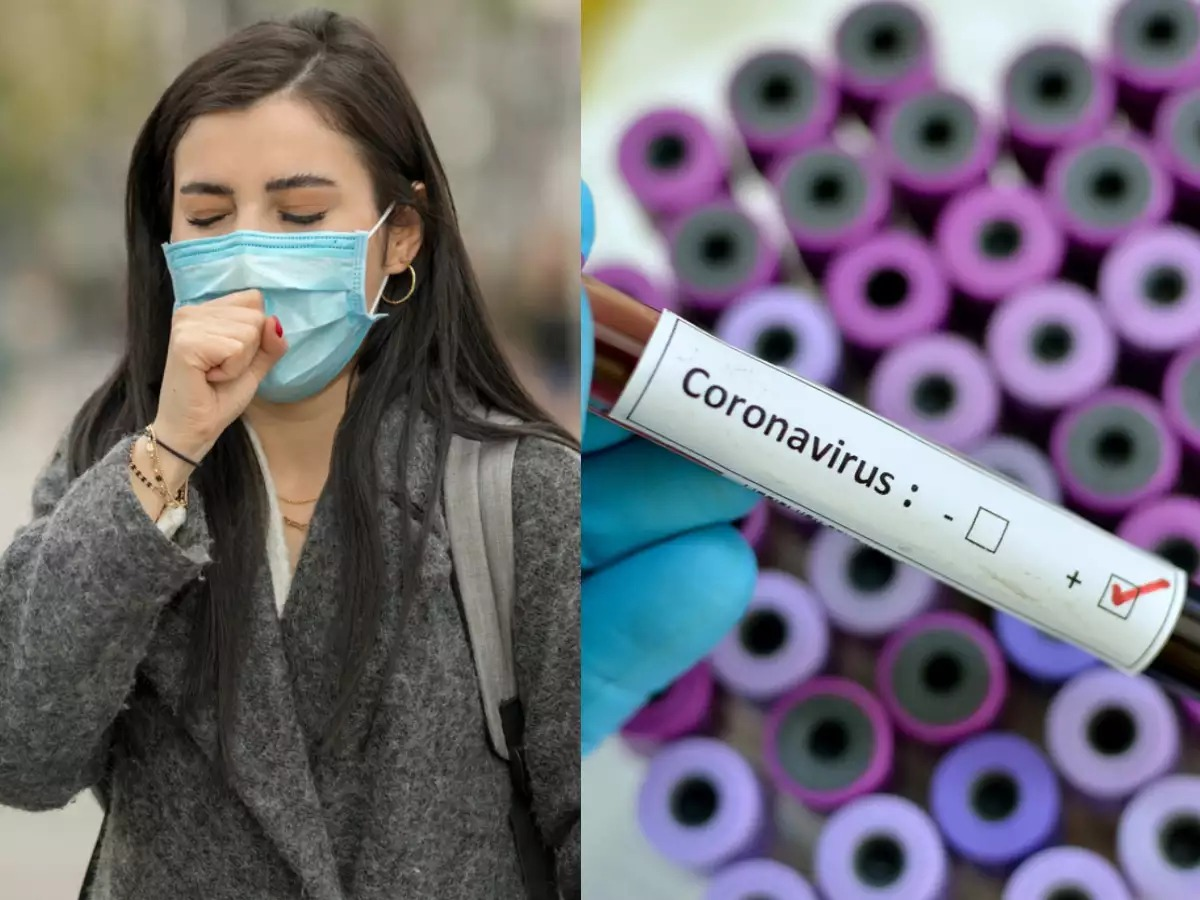
\includegraphics[width=\textwidth]{Intro.jpeg}\\
[2 cm]
\par 
In a Ted Talk delivered in 2014, Bill Gates warned that we were ill prepared for the next global catastrophic event, which he predicted would be from another uncontrolled viral epidemic.\\
\par And nowadays it became true becaue of global pandemiic \textcolor{red}{CORONA} virus.As we know,the World Health Organization (WHO) has declared the coronavirus disease 2019 (COVID-19) a pandemic. A global coordinated effort is needed to stop the further spread of the virus. A pandemic is defined as “occurring over a wide geographic area and affecting an exceptionally high proportion of the population.” The last pandemic reported in the world was the H1N1 flu pandemic in 2009.\cite{nj1}
\\
\par On 31 December 2019, a cluster of cases of pneumonia of unknown cause, in the city of Wuhan, Hubei province in China, was reported to the World Health Organisation. In January 2020, a previously unknown new virus was identified, subsequently named the 2019 novel coronavirus, and samples obtained from cases and analysis of the virus’ genetics indicated that this was the cause of the outbreak. This novel coronavirus was named Coronavirus Disease 2019 (COVID-19) by WHO in February 2020. The virus is referred to as SARS-CoV-2 and the associated disease is COVID-19.\cite{nj1}\\
\par There are many factors to see this world pandemic and save ourselves from this disease.Some steps can be taken by us to slow down its effect on our health.We all know some precautions which can be taken by ourselves like social distancing, hand sanatizing,wearing mask ,etc.But,you know why the respective government of any country frequently suggesting about all of these things?\\
\par How a particular area or city  has many cases of the disease and increases daily?We will try to know all these things by the SIR model and graph theory,where  we will come to know the exact reason and some solution to that problem.
 

\newpage
\section{The Application/Motivation}\label{sec:intro}
\begin{itemize}
\item As the title “\textcolor{red}{COVID-19}-\textcolor{blue}{The Global} \textcolor{red}{Epidemic}” suggests that the application is about present disease but this application is for all such global pandemic that had built a humanitarian crisis. We will see that how to stop the spreading of the disease and also measure the effect by Graph Theory and a model called SIR model.
\item The purpose to build this application is to overcome the effect of disease and bring our economy in a track by help of such an analysis of Graphs in the state, city, or some places.
\item By the application we will come to know that there are many applications of Graph theory and it is a very efficient and elegant method to describe connections of any type.
\\
[1.5 cm]
\underline{\bf\huge{Motivation}}
\item  I show a news channel daily and in the present time as we know the main headline of news is the spreading of COVID-19 disease. So, I thought to make an application based on this global pandemic.
\begin{center}
\includegraphics{Images.jpg}
\end{center}
\item Therefore, I have made it this application by using the concept of Graph theory and model called SIR model.
\end{itemize}

\newpage
\section{Formulation of the Mathematics}
\subsection{COVID-19 modeling by Graph theory}
\par  We all know our mind likes simplicity over hard things.So here,in \textcolor{blue}{Discrete Mathematics} we can define this disease by graph theory.
We can understand many concepts by graph theory simply and effectively.\\
\par  We can understand the situation and get solutions of this disease by graph theory.So,first understand it by asking questions:\\
\begin{enumerate}

\item {\bf{What is a social network}}
\end{enumerate}
\begin{figure}[h]
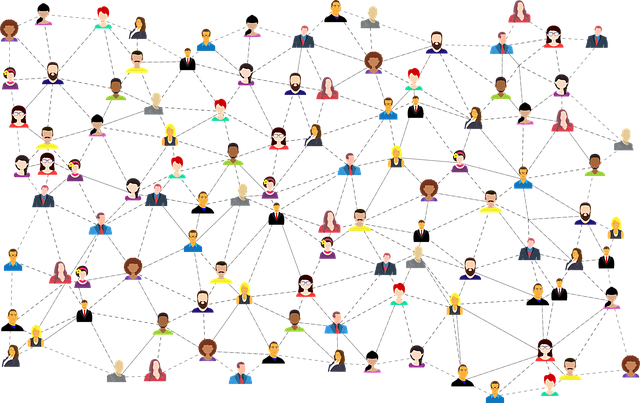
\includegraphics[width=\textwidth]{social-media-3846597_640.png}
\caption{Social network representation\cite{nj5}}
\end{figure}
\par Now,let's formulate one equation called maximum degree notation in Graph Theory for understanding connections.
\newpage
\begin{enumerate}
\item {\bf{What is Handshaking Lemma?}}
\\
[1 cm]
Handshaking lemma is about undirected graph. In every finite undirected graph number of vertices with odd degree is always even. The handshaking lemma is a consequence of the degree sum formula (also sometimes called the handshaking lemma)\cite{nj3}.
$$\therefore \boxed{\sum_{i=1}^{n} deg(V) = 2|E|}$$
\\
[1 mm]
\par Where,deg(V) is degree of vertex in a particular graph and E is the number of total edges in the graph.\\
[1 cm]

\textcolor{blue}{We derive equation of \textcolor{red}{ maximum degree} notation in following section.}
\\
[1 mm]
\item {\bf{Situation before spreading of disease}}

\begin{figure}[H]
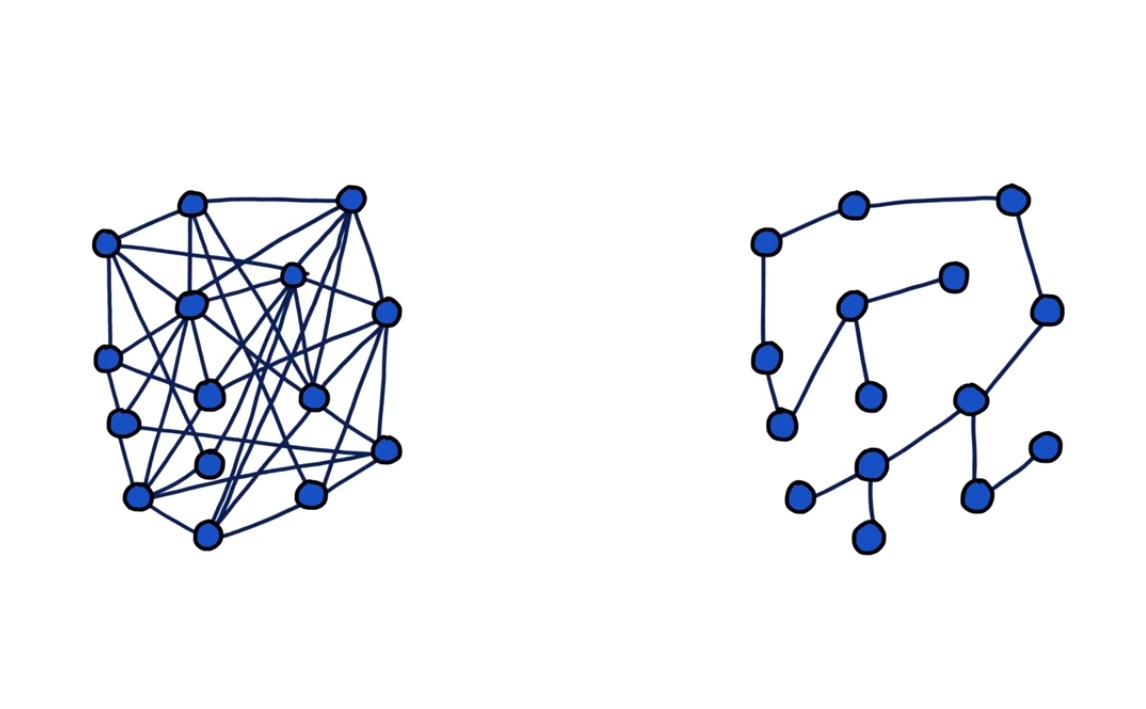
\includegraphics[width=\textwidth]{1st.jpeg}
\caption{Same number of nodes but pattern is different\cite{nj4}}
\end{figure}
\item {\bf{Situation after spreading of disease}}
\end{enumerate}
\begin{figure}[H]
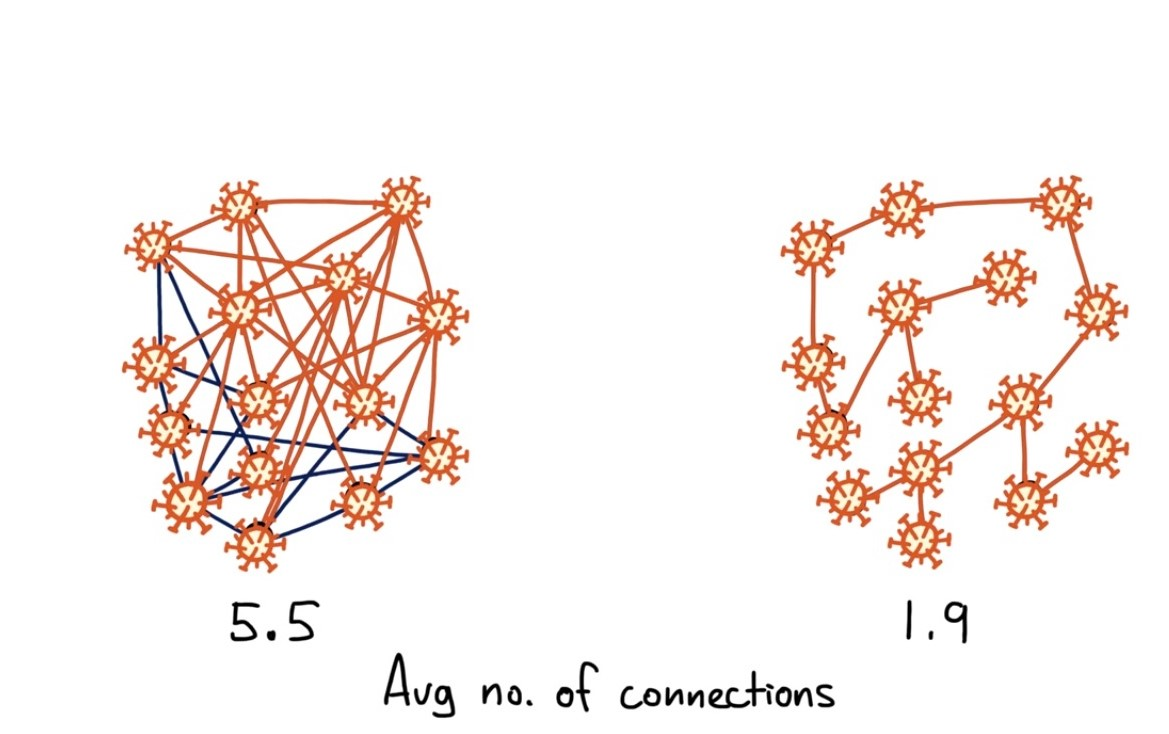
\includegraphics[width=\textwidth]{1st_condition_effect.jpeg}
\caption{Different effect on different patterns\cite{nj4}}
\end{figure}

\par Here,we can understand that by taking nodes as human being there are same number of nodes 16 but \textcolor{red}{one average person spread the disease to 5.5 in first graph and 1.9 in second graph}.
\\
So,we can say that the spread of virus is dependent on the {\underline\bf {pattern of the graph}}
\\
[1 cm]
\par Now,we understand the centrality concept for some glimpse of  \textcolor{red}{\underline{Super-spreaders}} effect on spreading the disease.\\

\begin{figure}[H]
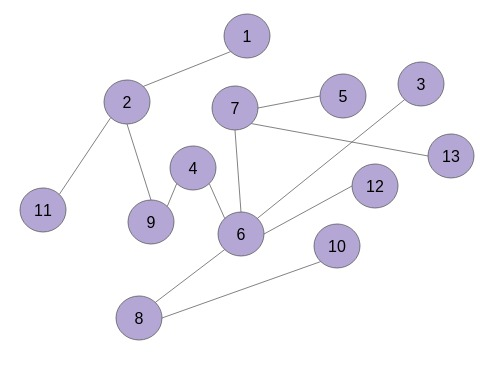
\includegraphics[width=10 cm,height=10 cm]{Cetrality.jpeg}
\caption{This figure shows connections to other nodes(human beings)\cite{nj5}
}
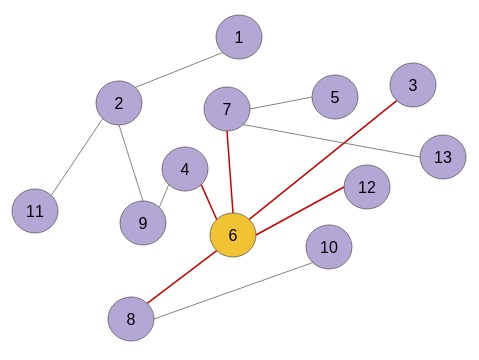
\includegraphics[width=10 cm,height=10 cm]{Cetrality_2.jpeg}
\caption{Node 6 is being detected as super spreader node(human being)\cite{nj5}}
\end{figure}

\par This can be detected by degree centrality method.This is shown below:\\
\begin{figure}[H]
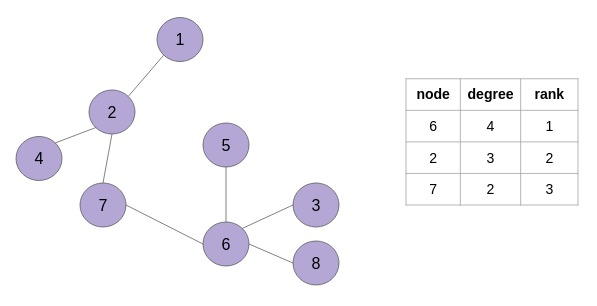
\includegraphics[width=10 cm,height=10 cm]{Centrality_3.jpeg}
\caption{Degree centrality\cite{nj5}} 
\end{figure}

\par We have formulated the mathematics of spreading of disease.Now,time is to get answers of following questions related to our topic graph theory in section:4.
\newpage


\subsection{Infectious Disease Modelling by SIR method}

\par I have found there is a simple mathematical model named SIR model describing the structure of how the infectious disease. The assertion by the model is so interesting to me even it is simple to explain. \\
[1 cm]
{\bf{ What is SIR model?}}\\
[5 mm]
SIR model is a kind of compartmental model describing the dynamics of infectious disease. You may wonder why it is called the “compartmental model.” The model divides the population into compartments. Each compartment is expected to have the same characteristics. SIR represents the three compartments segmented by the model.\cite{nj6}\\
[5 mm]
\begin{itemize}
\item\bf\textcolor{blue}{S}usceptible\\
\item  \bf \textcolor{blue}{I}nfectious \\
\item \bf \textcolor{blue}{R}ecovered\\
\end{itemize} 
\begin{figure}[h]
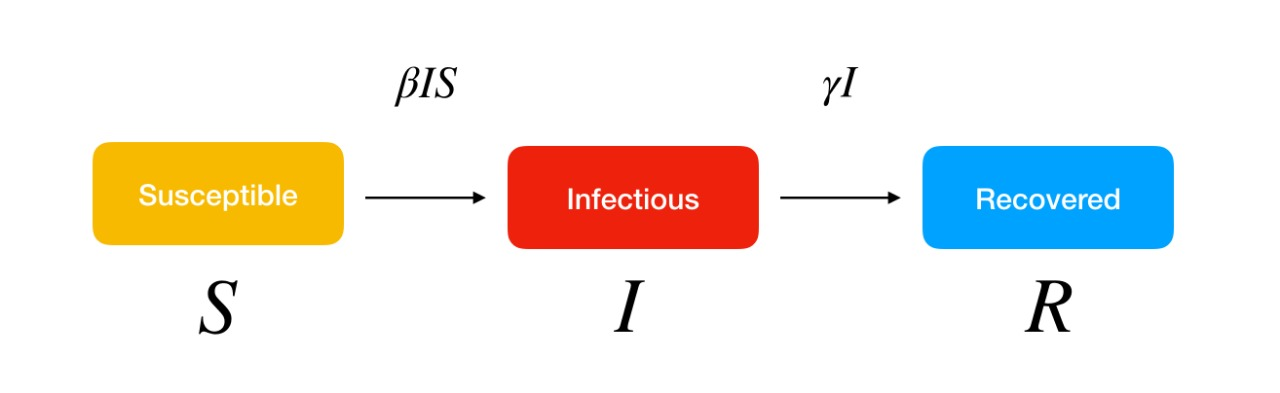
\includegraphics[width=\textwidth]{SIR.jpeg}\\
\caption{SIR MODEL\cite{nj6}}
\end{figure}

\newpage
SIR model allows us to describe the number of people in each compartment with the ordinary differential equation. 
$\beta$
 is a parameter controlling how much the disease can be transmitted through exposure. It is determined by the chance of contact and the probability of disease transmission. 
$\gamma$
 is a parameter expressing how much the disease can be recovered in a specific period. Once the people are healed, they get immunity. There is no chance for them to go back susceptible again.\\

\begin{equation}
\therefore\boxed{\frac{dS}{dt} =-\beta IS} \\
[1 cm]
\end{equation}
\\
\begin{equation}
\therefore \boxed{\frac{dI}{dt} =\beta IS-\gamma I} \\
\end{equation}
\\
[1 cm]
\begin{equation}
\therefore\boxed{\frac{dR}{dt} =\gamma I}
\end{equation}
\\
[1 cm]
\par  {\bf{Here,we can take this equation only by assuming this 3 things:}}\\

 {\huge \textcolor{blue}\bf{Assumptions:}}\\
\begin{enumerate}
\item Population remains constant
\item Rate of infectives \& contacts are prostional to each other
\item Infectives recovered or die at constant rate\\
\end{enumerate}
\par We can take,
\[S=S_0 \ \]\\
\[I=I_0  \]\\
\[R=0  \]
initially \\
[1 cm]
Also,we can say that:\\
\begin{equation}
\boxed{S+I+R=Total Population}\\
\end{equation}
\\[1 mm]
\begin{equation}
\boxed{S+I+R=\ S_{0}+\ I_{0}}  \\
\end{equation}
\par This equations are for initial condition.
\\[1 cm]
\par {\bf{Now we need to give the answer of the following questions:}}\\
\begin{enumerate}
\item\textcolor{blue}{ Will the disease spread?}\cite{nj8}
\item\textcolor{blue} {What is the maximum number of infectives?}\cite{nj8}
\item\textcolor{blue} {How many people  catch the disease?}\cite{nj8}
\end{enumerate}
\par \textcolor{black}{This questions lead us on the prevention of pendemic disease,which we will solve in Section:4.}\\
\newpage


\section{\bf {Solution  of the Mathematics}}




\subsection{ Solution to overcome the effect of disease by Graph Theory} 

\par {Here,we will  proove that  lockdown and Social distancing is very effective to reduce the effect of spreading by prooving the \textcolor{blue}{Maximum degree} notation.}\\
[1 cm]
By hand-shaking lemma,\\
$$\therefore \boxed{\sum_{i=1}^{n} deg(V) = 2|E|}$$
\\
[1 mm]
Now by above equation we get maximum degree,\\
\begin{equation}
\therefore\boxed {\Delta(G).|V| \leq2|E|}
\end{equation}
\\
[1 cm]
\begin{tcolorbox}[enhanced,fit to height=4cm,
  colback=yellow!25!black!10!yellow,colframe=green!75!white,title=\textcolor{red}{Conclusion:1},
  drop fuzzy shadow]
  \textcolor{blue}{\bf{By above equation,We can say that if we decrease the value of E means if we decrease the social contacts than the value of maximum degree is also decreased and therefore social distancing and self quarantine is much important by this sense.}} 
\end{tcolorbox}
\newpage
\par{ \bf{Here,we will try to answer the following questions:}\\
\begin{enumerate}
\item\textcolor{blue}{\bf {How can social network represented in graph theory help us to predict the spread of virus?}}
\item\textcolor{blue} {\bf{ How can graph theory inform our policies to help reduce spreading?}}
\end{enumerate}
\vskip 1.5 cm
\begin{enumerate}
\item{\bf\underline{ How can graph theory help us to predict the spread of virus?}}
\begin{figure}[H]
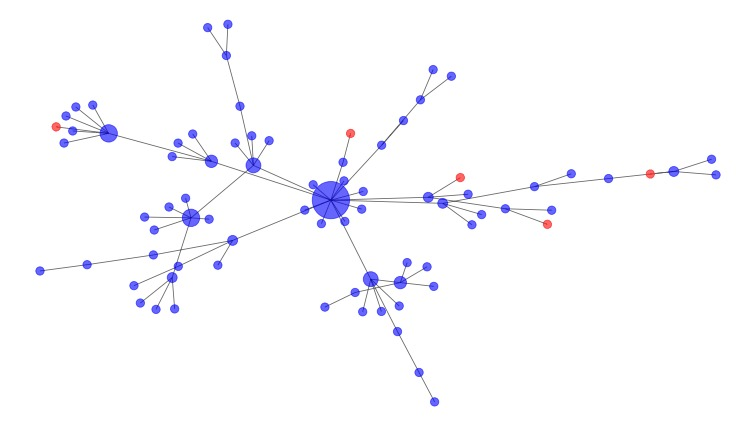
\includegraphics[width=\textwidth]{Socially.jpeg}
\caption{A connection of people to other nodes(people) before spread of virus(Consider as a city map node).\cite{nj7}} 
\end{figure}
\begin{figure}[H]
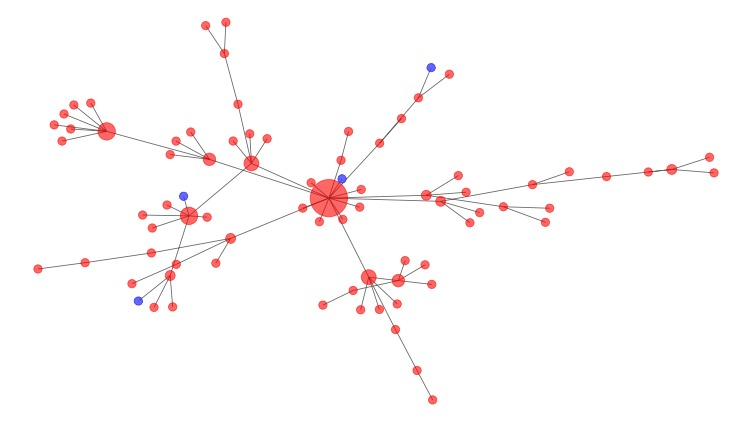
\includegraphics[width=\textwidth]{Sociallity_2.jpeg}
\caption{Red dots denote the infected people.\cite{nj7}} 
\end{figure}
\par Here in above Figure(9) big red dots are designated as \textcolor{red}{Superspreaders}.So we can reduce some effect of spreading the virus by quarantine them.As we quarantine them,the contact ratio is decreased and the node conneected to it is disconnected.So,we can save many lives from this work.\\

\begin{tcolorbox}[enhanced,fit to height=4cm,
  colback=yellow!25!black!10!yellow,colframe=green!75!white,title=\textcolor{red}{Conclusion:2},
  drop fuzzy shadow]
  \textcolor{blue}{Here,in above given figure connection pattern tells lots more about the Susceptible and infectives .This is the main reason that why particular area or city has more cases of virus than other.} 
\end{tcolorbox}
\newpage
\item{\underline{\bf{ How can graph theory inform our polices to help reduce spreading?}}}
\\
\par Our polices can detect this spread of disease by help of Graph theory.The main aspect to reduce the number of cases is t find the \textcolor{red}{Superspreaders}.This can be done by countinfg the degree of the nodes.A node with higher degree can spread the disease in big amount.So,first task is to find them.
\\
\par The second aspect is \textcolor{blue}{Social distancing} to decrease our contact ratio designated in above subsection.This can be also see by Graph theory.\\

\begin{figure}[H]
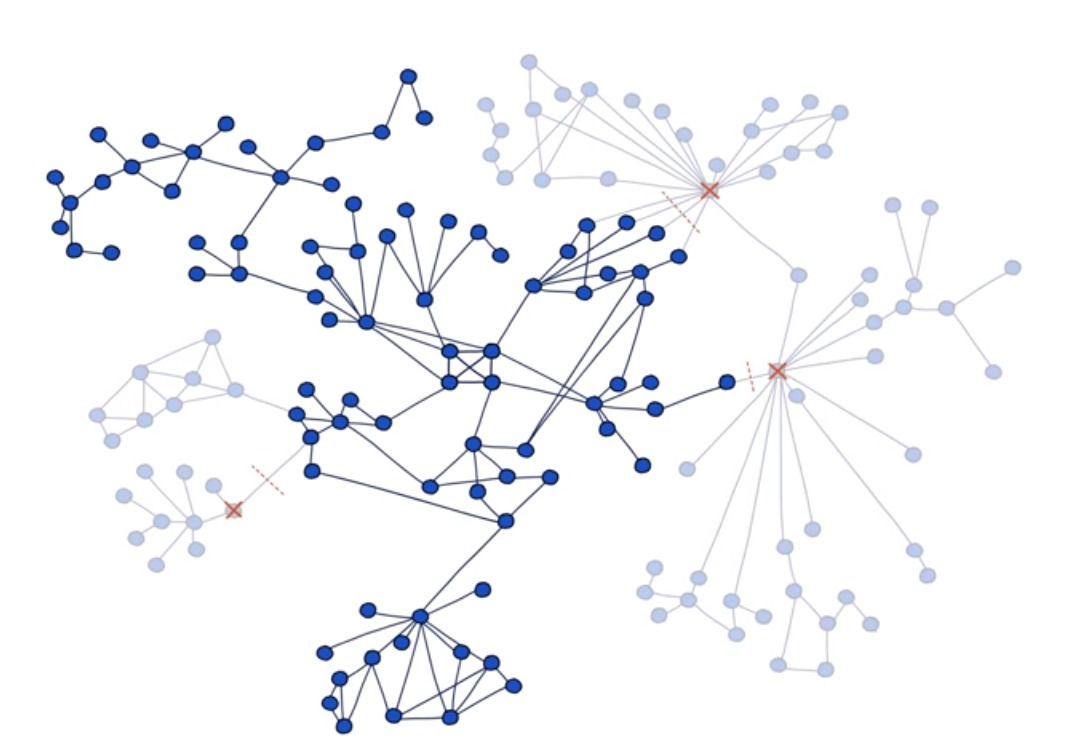
\includegraphics[width=\textwidth]{quarantine (2).jpeg}
\caption{The effect of self quarantine or lockdown.}
\end{figure}
\begin{tcolorbox}[enhanced,fit to height=4cm,
  colback=yellow!25!black!10!yellow,colframe=green!75!white,title=\textcolor{red}{Conclusion:3},
  drop fuzzy shadow]
  \textcolor{blue}{We show many aspects to decrease the cases of virus and learn that the disease spread is dependent upon the pattern of graph in any city or place so government has to prepare stratagy by looking this pattern and than implement ideas on the basis of this method.This is very effective measure of spread of disease.} 
\end{tcolorbox}

\end{enumerate}
\newpage

\subsection{ Solution to overcome the effect of disease by SIR model theory}
\begin{itemize}
\item We ask following question in above section:
\end{itemize}
\begin{enumerate}
\item\textcolor{blue}{\bf  Will the disease spread?}\cite{nj8}
\item\textcolor{blue} {\bf What is the maximum number of infectives?}\cite{nj8}
\item\textcolor{blue} {\bf How many people  catch the disease?}\cite{nj8}
\end{enumerate}
\begin{enumerate}
\item{\bf\underline{Will the disease spread?}}\\
\par We got  this equation in previous section:
$$\frac{dI}{dt} =\beta IS-\gamma I $$
\\
Now as we know,
\begin{equation}
S\leq\ S_{0}
\end{equation}
\begin{equation}
\therefore \boxed{\frac{dI}{dt}< I[\beta \ S_{0}-\gamma]}
\end{equation}
\par By Eq.(7) we can get some parameters and we can say that:\\
\begin{equation}
 \boxed{\ S_{0}>\frac{\gamma}{\beta}=\frac{1}{q}}\cite{nj8}
\end{equation}
\\
where q is a contact ratio.

 if above inequality satisfies than  the disease willl spread.
\\
by this we can get ,\\
\begin{equation}
\ R_{0}=\frac{\beta \ S_{0}}{\gamma}
\end{equation}
\par This ratio is very important and called basic reproduction number defined as the expected number of secondary cases produced by a single (typical) infection in a completely susceptible population.
\\
[0.5 cm]
\begin{figure}[H]
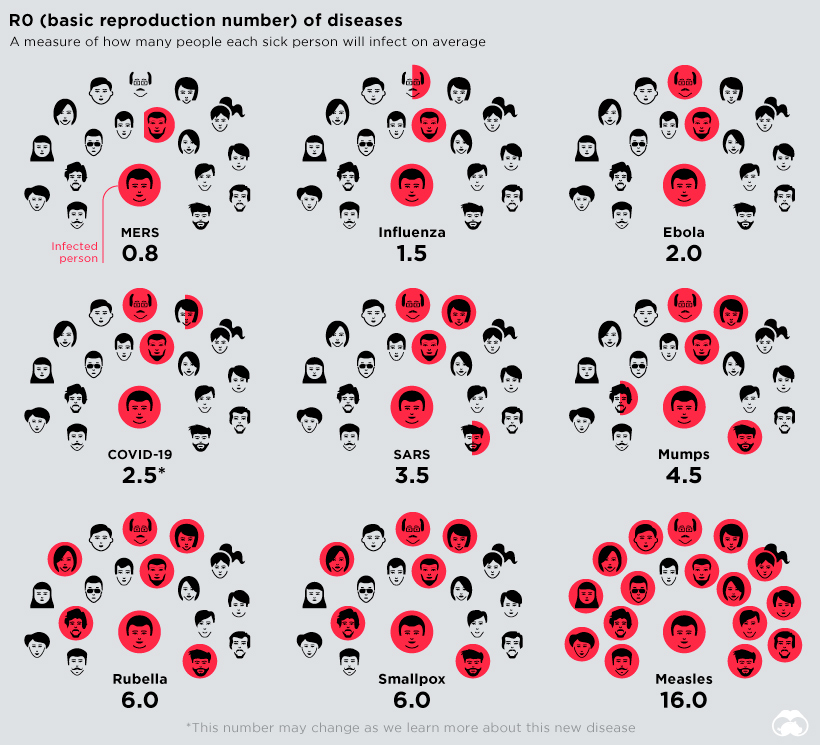
\includegraphics[width=15 cm,height=10 cm]{deadliest-pandemics-R0-disease-spread.jpg}
\caption{Past  pendemics basic reproduction numbers.}
\end{figure}
\par Scientists use a basic measure to track the infectiousness of a disease by $\ R_{0}$. 
\\
[1.5 cm]


\begin{tcolorbox}[enhanced,fit to height=4cm,
  colback=yellow!25!black!10!yellow,colframe=green!75!white,title=\textcolor{red}{Conclusion:1},
  drop fuzzy shadow]
  \textcolor{blue}{If the ratio is $>$1 than the disease is called global pandemic as the corona virus is declared.For COVID-19 the ratio is about 3 to 4.\\ Also the spread of disease is dependent upon the contact ratio q that we will see in the next question.} 
\end{tcolorbox}
\newpage


\item{\bf\underline{What is the maximum number of infectives?}\cite{nj8}}
\\
For find $\ I_{max}$,\\
[1 cm]
$$\therefore \frac{dI}{dS}=\frac{\beta IS-\gamma I}{-\beta IS}$$\\
[0.5 mm]
$$\therefore \frac{dI}{dS}=-1+\frac{\gamma}{\beta S}$$
\\[0.5 mm]
\begin{equation}
\therefore \boxed{\frac{dI}{dS}=-1+\frac{1}{qS}}
\end{equation}
\par Now $$S+I+R=\ S_{0}+\ I_{0}$$
\\
[0.5 mm]
\begin{equation}
\therefore I+S-\frac{1}{q}\ln{S}=\ S_{0}+\ I_{0}-\frac{1}{q}\ln{\ S_{0}}
\end{equation}
\begin{equation}
\therefore \boxed{\ I_{max}=\ S_{0}+\ I_{0}-\frac{1}{q}[1+ln({q\ S_{0}})]}\cite{nj8}
\end{equation}
\\

\begin{tcolorbox}[enhanced,fit to height=4cm,
  colback=yellow!25!black!10!yellow,colframe=green!75!white,title=\textcolor{red}{Conclusion:2},
  drop fuzzy shadow]
  \textcolor{blue}{So,by above $\ I_{max}$ equation we can conclude that if our contact ration is high than there are more affected person and therefore \textcolor{blue}{Lockdown is very important to no spread the disease and decrease the contact ratio.}} 
\end{tcolorbox}





\item{\bf\underline{How many people can catch the disease?}}\cite{nj8}
\\
[1 cm]
As we know initially that,
$$S+I+R=\ S_{0}+\ I_{0} $$ \\
\begin{equation}
\ R_{end}=-\ S_{end}+\ S_{0}+\ I_{0}
\end{equation}\\
[0.5 mm]
\begin{equation}
\therefore \boxed{\ S_{end}-\frac{1}{q}\ln{\ S_{end}}=\ S_{0}+\ I_{0}-\frac{1}{q}\ln{\ S_{0}}}\cite{nj8}
\end{equation}
\\


\begin{tcolorbox}[enhanced,fit to height=4cm,
  colback=yellow!25!black!10!yellow,colframe=green!75!white,title=\textcolor{red}{Conclusion:3},
  drop fuzzy shadow]
  \textcolor{blue}{So,here $\ S_{end}$ people can catch the disease and it's also dependent upon contact ratio q if q value is much bigger that much people are being infected that is obvious and we can say it also by looking at equation.} 
\end{tcolorbox}




\end{enumerate}

\newpage

\section{Interpretation and significance of the solution for application}

\begin{itemize}
\bf \huge{\item \underline{ Interpretation}}
\end{itemize}
\vskip 1 cm


\begin{itemize}
\thispagestyle{empty}
\item  As we know that the corona virus has affected on global economy and mankind. As the virus spreads all over the world, number of infectives increases day by day, so many country’s government has declared lockdown for several days. But as we know it also effect on economy.
\item So, there are two main problem for governments how to save the country economically and socially.But every problem has its solution. As per my application I have formulated it by Graph Theory and SIR model.
\item Here, SIR model is mainly used because of derivation of basic reproduction number R0. Most of tracking of virus spread has been done by this notation. Also, maximum number of infectives can be find by this SIR model. By seeing eq.(13) one can conclude that it’s depends on contact ratio (q) means contact to another person.
\item	There are many uses of Graph theory to measure and reduce the effect of disease. In my application by using Handshaking Lemma I have found max degree notation $\Delta (G)$  in eq.(6).By this equation we are come to know that how Social distancing help us to reduce the effect of disease.
\item 	By Graph theory we can easily find out the connection to that Super spreaders and immediately break the chain of virus by quarantine them. This has been shown in Fig.(10).
\item	I have answered the questions shown below:
\begin{enumerate}
\item  How can social network represented in graph theory help us to predict the spread of virus?
\item  How can graph theory inform our polices to help reduce spreading?
\end{enumerate}
\par This all can be happened by using Graph theory in my application.
\vskip 1.5 cm
\begin{itemize}
\bf \huge{\item \underline{Significance}}
\end{itemize}
\vskip 1 cm

\item 	In which place lockdown must be remain and in which place some relief should be given can be decided by this Graph theory.
\item As per one example let’s assume that any two city A $\&$  B has same population but by representing them using graph City A has dense graph and city B has sparse graph. So, how number of cases increases day by day in City A can be thought by this pattern.
\item 	By this we come to know that in city B there are chances that cases will not increase as increase in City A. So, some relief should be given in City B.
\item 	Using this technique, we can stop to spread the disease in some extent and also bring the economy in its track.
\\
[1.5 mm]
\begin{center}
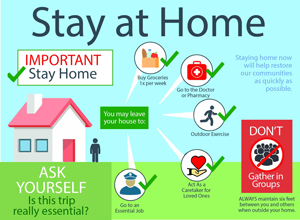
\includegraphics{Document.png}
\end{center}
\end{itemize}
\newpage
\section{Commercialization}
\vskip 1 cm
\begin{itemize}
\item I can make an app which will use Google map. If a person has a work like buying vegetables or medicine or another important work like visiting bank, then during such crisis person has to make sure that he must not go to that area which has more positive cases of virus. My app will warn that person, if he is nearby to that area or zone or more infected people. This app will help people to not spread the virus and save themselves from the virus.
\\
[1 cm]
\textcolor{red}{If I will start my own company than my dream logo will look like this}:
\begin{center}
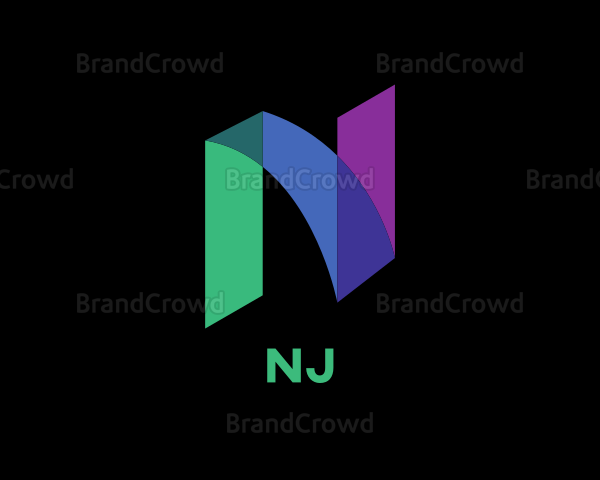
\includegraphics[width=5 cm,height=5 cm]{large.png}
\end{center}
\item By using this application I can start up my own business and work as a technical$\backslash$professional consultant. In this post, I can analyze the effect of disease, the spread of disease, and the most important Super spreaders of the disease. This can any type of disease which can be spread by contacts. This has been done by some tracking methods that have been designated in this application. By the further study of such type of application this can also be used for predicting the effect of disease. So with the help of it the government can take some early precautions for it and save mankind and also economy from the disease.
\end{itemize}
\newpage
\addcontentsline{toc}{section}{\numberline{}\textcolor{red}{\bf{References}}}
\bibliographystyle{plain}
\bibliography{201901026}
\end{document}
